\documentclass{report}
\usepackage[]{algorithm2e}
\usepackage[utf8]{inputenc}
\usepackage[T1]{fontenc}
\usepackage[frenchb]{babel}
\usepackage{amssymb}
\usepackage{amsmath}
\usepackage{mathtools}
\usepackage{bbm}
\usepackage{listingsutf8}
\usepackage{verbatim}
\usepackage{xcolor}
\usepackage{graphicx}
\usepackage[toc,page]{appendix}

\lstloadlanguages{R}
\DeclareMathOperator*{\argmax}{arg\,max}

\begin{document}
\lstset{
    language=R,
    basicstyle=\footnotesize,
    numbers=left,
    backgroundcolor=\color{white},
    breakatwhitespace=false,
    breaklines=true,
    captionpos=b,
    commentstyle=\color{green},
    extendedchars=true,
    keepspaces=true,
    keywordstyle=\bfseries\color{blue},
    numbersep=5pt,
    numberstyle=\tiny\color{gray},
    showtabs=false,
    stringstyle=\color{red},
    tabsize=2,
    title=\lstname
}

\title{SY09 - TP4 Challenge Spam}
\date{Juin 2016}
\author{Stéphane LOUIS et Paul GOUJON}
\pagenumbering{gobble}
\maketitle

\newpage
\tableofcontents{}

\newpage
\pagenumbering{arabic}
\chapter{Introduction}

\paragraph{Objectifs}
L'objectif principale de ce sujet challenge est de nous "mettre dans la peau" du Data Scientist ayant à effectuer un choix de classifieur parmi un certain nombre de classifieur qu'il connait, dans le but de réaliser des tâches de discrimination sur un jeu de données réelles inconnu. Pour ce faire, nous allons découper notre étude en trois parties :

\begin{enumerate}
    \item Etude des caractéristiques générales de l'échantillon
    \item Etude des performances des classifieurs du TP4 sur l'échantillon
    \item Travail succint de veille sur les techniques actuelles de spam filtering
\end{enumerate}

\chapter{Etude}

\paragraph{Introduction}
Nous allons tenter de déterminer une stratégie permettant de discriminer les données spam. Pour cela nous commencerons par étudier les caractéristiques générales du jeu de données, puis testerons les performances des différents classifieurs programmés au cours du TP4 sur le dataset, avant d'exposer quelques résultats d'une étude de litterature que nous avons menée sur internet concernant le filtrage de spam.

\section{Caractéristiques générales du dataset}
\paragraph{Introduction}
Commençons par étudier quelques caractéristiques générales du jeu de données.

\paragraph{Corrélation}
Intéressons nous dans un premier temps au degré de corrélation des variables du jeu de données. Pour cela nous dessinons la heatmap représentant la corrélation entre les différentes variables du dataset.

\begin{figure}[ht!]
\begin{center}
    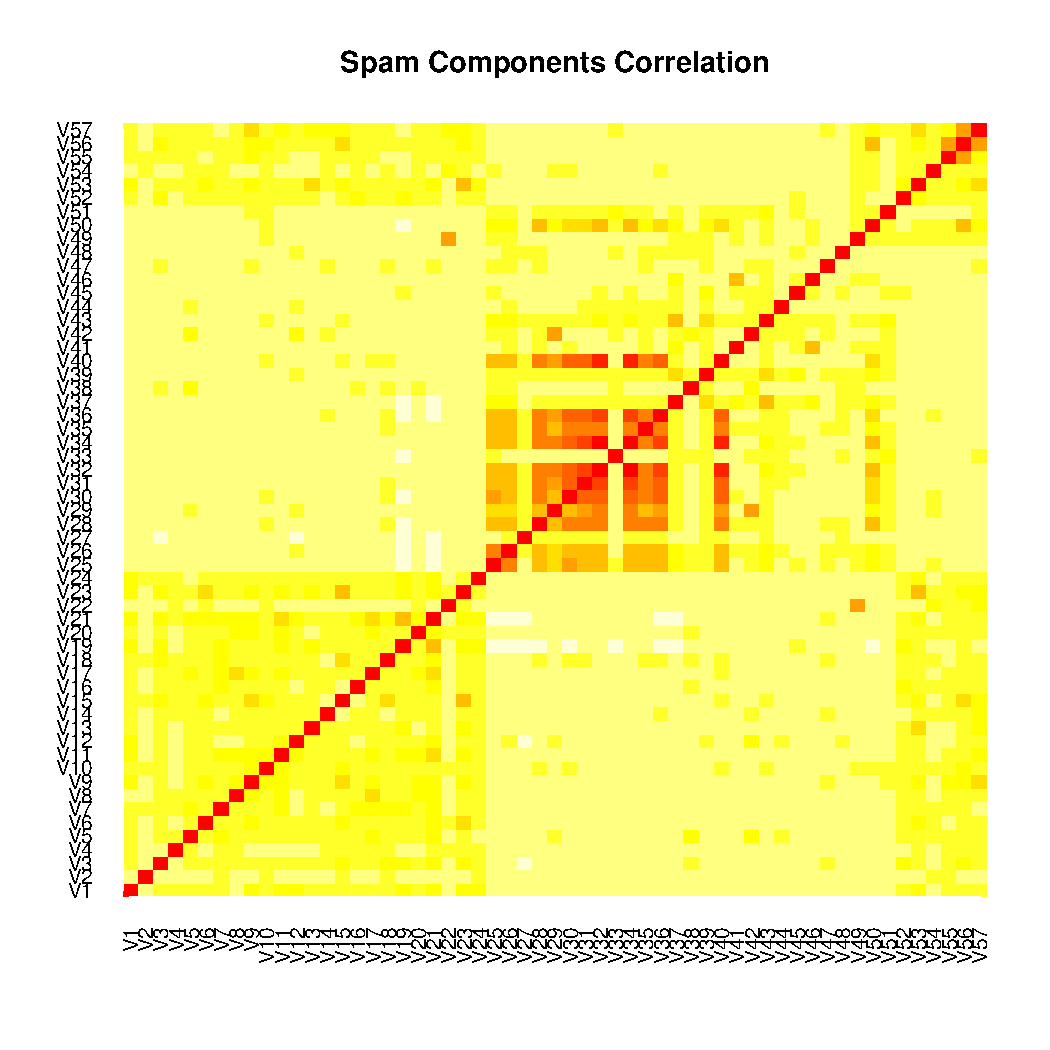
\includegraphics[width=\textwidth]{component_cor.pdf}
    \caption{Heatmap représentant la corrélation entre les différentes variables du jeu de données}
\end{center}
\end{figure}

\clearpage
\paragraph{Interprétation}
Sur la heatmap, plus les couleurs sont proches du rouge, plus la corrélation est proche de 1, plus les couleurs se rapprochent du blanc, plus la corrélation est proche de 0. Cette méthode de data visualisation nous permet de voir que les variables du dataset sont relativement peu corrélées. Il semble donc qu'elles apportent toutes une certaine quantité d'information, et doivent donc toutes être prises en compte pour l'établissement d'un modèle.

\paragraph{ACP}
Comme tout bon étudiant de SY09, nous avons eu immédiatement envie de voir s'il était possible de tirer des conclusions d'une ACP effectuée sur les données spam. En voici le tracé sur le premier plan factoriel :

\begin{figure}[ht!]
\begin{center}
    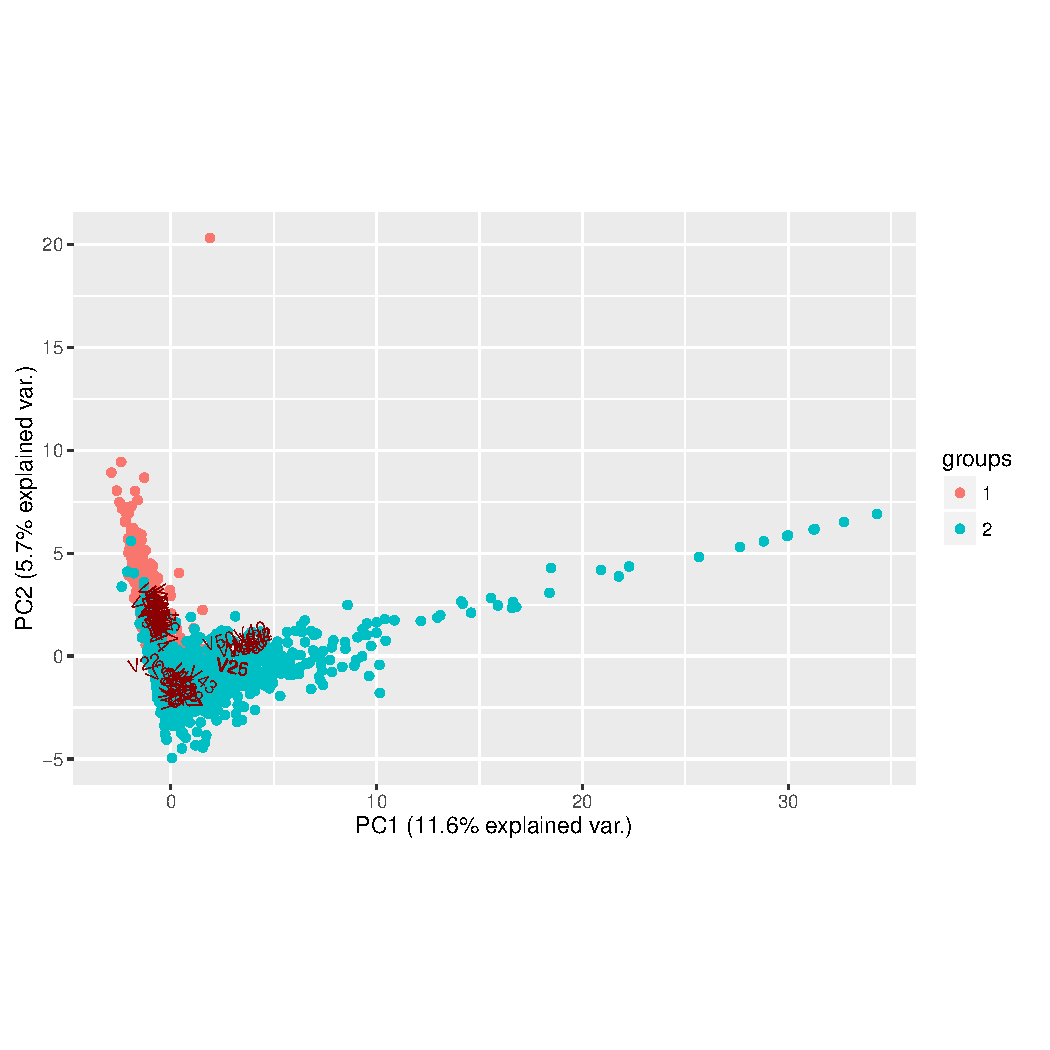
\includegraphics[width=\textwidth]{pca_spam.pdf}
    \caption{Tracé dans le premier plan factoriel de l'ACP effectuée sur le jeu de données spam}
\end{center}
\end{figure}

\paragraph{Interprétation}
Comme nous pouvons le voir, les pourcentages d'inertie expliquée par les axes du premier plan factoriel sont assez faibles, et de manière plus globale, il faut prendre en compte un grand nombre de composantes principales pour atteindre un niveau d'inertie expliquée convenable. L'intérêt d'étudier les données dans le premier plan factoriel est donc extrêmement limité et nous ne nous y attarderons pas.

\paragraph{Caractéristiques générales}
L'étude du retour de la fonction \verb+summary(X)+ ne donne pas beaucoup plus de résultats, très peu d'informations donnant matière à interprêter.

\paragraph{Conclusion}
Il est donc difficile, après cette première étude du jeu de données de formuler la moindre hypothèse à propos de la distribution des individus au sein de l'échantillon.

\section{Tests des classifieurs du TP4}
\paragraph{Introduction}
Suite à cette étude préliminaire du jeu de données assez peu fructueuse en terme d'hypothèse formulées concernant le choix de classifieur à effectuer, nous passons dans une second temps à l'étude des performances de nos classifieurs via l'estimation de leur taux d'erreur $\varepsilon$ et les intervalles de confiance correspondants.

\paragraph{Résultats}
Les classifieurs que nous avons implémentés fonctionnent sans problème sur ce jeu de données, et les résultats que nous obtenons sont les suivants:

\begin{table}[h!]
    \centering
    \caption{Estimations des taux d'erreurs et intervalles de confiances, par classifieur, sur le jeu de données "spam"}
    \label{tab:table1}
    \def\arraystretch{1.5}
    \begin{tabular}{c||c|c|c}
        \hline
        & ADQ & ADL & NBA\\
        \hline
        $\varepsilon$ & 0.168 & 0.112 & 0.113\\
        \hline
        $IC$ & $[0.157 ; 0.179]$ & $[0.103; 0.121]$ & $[0.104 ; 0.122]$\\
        \hline
        \hline
        & LOGBT & LOGBF & TREE\\
        \hline
        $\varepsilon$ & 0.068 & 0.076
        & 0.032\\
        \hline
        $IC$ & $[0.060 ; 0.075]$ & $[0.069 ; 0.084]$
        & $[0.026 ; 0.037]$\\
        \hline
        \hline
    \end{tabular}
\end{table}

\paragraph{Interprétation}
Nous obtenons les meilleures performances dans le cas de l'arbre de décision. Vient ensuite la Regression Logistique, et pour finir les classifieurs de l'Analyse Discriminante. Nous pouvons émettre l'hypothèse que les classifieurs de l'Analyse Discriminante produisent les moins bons résultats du fait de la non correspondance entre la distribution des données du jeu de données et les hypothèse assumées comme vérifiées par ces classifieurs. Cela expliquerait également, les relativement bons résultats de la Regression Logistique, ne reposant pas sur ces hypothèses (cas Gaussien, homoscédasticité, indépendance conditionnelle des variables...), se montrant ainsi plus robuste. Finalement nous constatons que l'arbre de décision fournit de très bonnes performances, mais nous soupsonnons que cela soit lié au fait que nous ayons testé les performances de ce classifieur sur nos données d'apprentissage : l'arbre de décision délimitant l'espace des individus en sous-régions de décision, s'adapte à nos individus d'apprentissage et fournira logiquement de bonnes performances pour la classification de ces derniers. Nous pourrions nous attendre à de moins bonnes performances sur des individus n'ayant pas servi à l'apprentissage.

\section{Etude de la litterature}
\paragraph{Introduction}
Pour finir, nous nous sommes intéressé à l'état de l'art en matière de "spam filtering", afin de voir les méthodes les plus utilisées dans le cas de la détection de spam de nos jours. Plusieurs méthodes ressortent très souvent.

\paragraph{Naive Bayes spam filtering}
Ce classifieur considère un mail comme un "sac de mots" (bag of word en anglais), c'est à dire ne considère pas la structure de ce dernier mais simplement le nombre d'apparition de certains mots en particulier. En fonction de cette mesure du nombre d'occurence de certains mots, le classifieur, suivant les préceptes du Théorème de Bayes, estime la probabilité que l'email soit du spam ou non. Bien que nous ayons obtenus des performances limitées pour le NBA au cours de notre expérimentation, il semblerait que cette technique demeure l'une des plus utilisées, aujourd'hui encore.

\paragraph{Support Vector Machine}
En machine learning, les SVM (Machines à vecteurs de support ou séparateurs à vaste marge en français) sont un ensemble de techniques d'apprentissage supervisé destinées à résoudre des problèmes de discrimination et de régression. Le modèle SVM choisit une frontière de décision maximisant la marge, c'est à dire la distance entre la frontière de décision et les échantillons les plus proches. Afin de pouvoir traiter le cas où les données ne sont pas linéairement séparables, les SVM tranforment l'espace de représentation des données d'entrée en un espace de plus grandes dimensions. Ceci est réalisé grâce à une fonction noyau, qui doit respecter les conditions du théorème de Mercer, et qui a l'avantage de ne pas nécessiter la connaissance explicite de la transformation à appliquer pour le changement d'espace. Les SVM reformulent ainsi le problème de discrimination en un problème d'optimisation quadratique. L'idée dans le cas de la classification en spam / non spam va de nouveau consister à utiliser l'approche "bag of word" appliquée aux emails, afin d'en tirer des vecteurs de caractéristiques, puis d'apprendre un modèle SVM permettant de les discriminer. Cette méthode produit apparemment de très bons résultats.

\paragraph{Perceptron}
Le perceptron est un algorithme effectuant l'apprentissage d'un classifieur binaire prenant comme valeur d'entrée un vecteur réel $x$, et retournant une valeur binaire $f(x)$ :


$$f(x) =
    \begin{cases}
        1, & \text{si } w.x + b > 0 \\
        0, & \text{si } sinon
    \end{cases}
$$

avec $w$ un vecteur de poids et $w.x$ le produit scalaire $\sum_{i=1}^m w_i x_i$, $m$ le nombre de d'entrées du perceptron et $b$ le biais. Une nouvelle fois, l'approche pour la discrimination d'email consiste à considérer ces derniers suivant l'approche "bag of words", et s'intéresser au nombre d'occurences d'un certain nombre de mots, vecteur d'occurences qui sera fourni en entrée au perceptron. Les performances du perceptron serait, d'après les articles que nous avons consultés, encore meilleures que celles du modèle SVM.

\chapter{Conclusion}

\paragraph{Conclusion}
Ce sujet challenge a été pour nous l'occasion de se "mettre dans la peau" du Data Scientist qui aurait face à lui un jeu de données réelles et pour lequel il devra choisir un modèle de discrimination. Nous avons vu qu'il était bien plus difficile de déterminer par des méthodes "basiques" les caractéristiques générales d'un échantillon, ou les hypothèses qui peuvent être assumées comme vérifiées ou non. Nous avons par conséquent évalué les performances de nos classifieurs via l'estimation de leurs taux d'erreurs et les intervalles de confiance correspondant. Finalement, nous avons effectué un court travail de veille, nous ayant permis de nous renseigner sur "l'état de l'art" dans le domaine du spam filtering.





\end{document}
